\section{Implementation of Game Software}

This section deals with the implementation of the modules discussed in the design section.
Since it is pointless to describe exactly how the code performs its function, as this 
can be read directly from the code, it is described what the code does in  broad terms and why. 

\subsection{Hardware Abstraction Layer Implementation}
As mentioned before, the hardware layer is fairly thin as only three modules are needed for our game.

\paragraph{SPI module}
The setup\_SPI\_master() function  configures the hardware SPI module the eZ8 development board to run at max speed as a master.
The write\_spi() pulls the slave pin low, signaling the start of a transmission and places its argument in the SPI data register
which immediatly starts transferring the data. It then waits until the transmission is complete and returns.
The source is found in spi.c/h.

\paragraph{Timerlib}
The set\_timer() functions takes arguments to configure what timer to enable, what period the timer
should be set to, the priority, and what function should be called when the interrupt occurs. Currently
only one timer can be enabled and the timer select argument is simply ignored, so is the priority. 
The function calculates the needed reload values for the timer and enables TIMER0. The interrupt vector
is set to call a function which immediately calls the function passed as an argument using a function pointer.
The source is found in timerlib.c/h.

\paragraph{ADC input}
the ADC module is fairly simple. The setup\_joystick() function takes
no arguments and configures the PB0 pin on the eZ8 development board for its alternate ADC function.
The read\_joystick() function simply returns the most significant 8 bits of the current ADC sample.
The source is found in joystick.c/h.

\subsection{API Layer Implementation}
The API layer uses the functions provided by the hardware abstraction layer to present additional functionality to the application
layer.

\paragraph{Input Module}
The input module manages and presents a global array to the application layer. This global array contains the state of all inputs
and it is updated every time get\_input() is called. The array indexing is managed with an enumeration, such that
additions to the array do not destroy existing dependencies. The array is global because almost every module in the
application layer needs access to the current keystate or joystick value. The input array is only updated by the 
input module. Before being able to utilize joystick input, an application must first call setup\_input() which 
makes sure that the joystick ADC pins are enabled. The source is found in input.c/h.

\paragraph{Sound Module}
The sound module contains different named sounds that can be played by calling the play\_sound() function.
To be able to play sound, the SPI module must first be setup and so the sound module includes a
function for enabling the sound. The source is found in sound.c/h.

\paragraph{Math module}
The math module contains a macro for the cosine function and 8.8 fixed point math. Its only real
function is the sin() function. This takes an argument in 512-degrees and returns the
sine value of the angle from a lookup-table that was generated by an excel macro given in
the first weeks exercises. The source is found in math.c/h.

\paragraph{Timekeeping Module}
The timekeeping module simple calls through to the hardware layer to set up a timer. The source is found in
timekeeping.c/h

\paragraph{Graphics Module}
The graphics module utilizes the UART on the eZ8 board to send ANSI escape codes to a terminal on a PC.
The gotoxy(), clrscr() and color change functions simply send an ANSI escape code using printf() from 
the eZ8 stdlib. The set\_monochrome() and set\_background() functions manage a set of variables
that are global to the graphics.c file scope and not to the entire program. These are used by
the background drawing functions that calculate what color to place behind characters being drawn.
Changing the color for every character is extremely bandwith intensive, and therefore the current
color is kept track of by another set of locally global variables such that color change messages
only need to be sent when actually necessary. When the monochrome variable is set to true, all
images are drawn in black and white only. The source is found in graphics.c/h  

\subsection{Application Layer Implementation}
The application layer exclusively uses API functions to perform the game simulation and updating.

\paragraph{Main function}
The main function initialises the inputs, outputs, and the timer needed for the application. After this
it uses helper functions to start the game. Every time the timer fires an interrupt, a global update flag
is set to true which triggers updating and rendering of all entities as shown in figure \ref{top_flow}.
The main function acts as the state manager in the block diagram shown in figure \ref{architecture_block}

\paragraph{Levels Module}
The levels module contains all the game levels. These are represented as a struct that contains
information about how many bricks the level contains, which is needed for the bricks array
that holds all the bricks that need to be updated. The struct also contains the brick layout
for generating the brick entities in the right positions and a pointer to a background pointer, 
which is used for the load\_level() and end\_level() helper functions that display the background
image. The levels module holds a global variable used at the top level, the current level. The source
is found in levels.c/h.

\paragraph{Backgrounds module}
The backgrounds module contains constant arrays of generated ASCII art data. These arrays are used
to display the level backgrounds and are generated using a java program that transform a raster
art picture to ASCII art. The module also contains pointers to these constant arrays. Every
background takes up 8KB of space and is therefore saved in the ROM by enabling the compiler
directive that places all constant variables in ROM. Source is found in backgrounds.c/h.

\paragraph{Entities}
All entities use the same basic blueprint. A struct containing the variables that they can share
with other entities, position fields always in 8.8 fixed point format, function pointers
 to their specific render, update and collided functions, and
a void pointer to a struct containing encapsulated data that is only used by the entity itself. 
Using the void pointer makes it harder for other entities to use the data encapsulated in the
struct pointed to by the void pointer, which helps to avoid interdependencies. Every entity also
has a create and destroy function which makes it possible to allocate memory for the entity
and free it upon destruction. This needs to be done to avoid the entities going out of scope
and their data being overwritten. The function pointers to update, render and collided functions
makes the code at the top level clearer and easier to extend since the internal functions that
are pointed to can be changed at will without changing other code.

\paragraph{Ball Entity}
As the ball is the only entity that can collide with other entities, this entity provides its own 
collision detection, other entities simply employ boundary checks. The collision checking code
uses and ID passed to it to determine which entity the ball is currently checking against.
This allows the ball to act uniquely depending on which entity it collides with.
 The ball also holds the score
as it is convenient to represent the player as the ball instead of the striker. The ball
uses a polar representing of its velocity and angle such that it can move in any direction
and reflection calculations are easy to perform. A flowchart of the
 code called when a collision has been detected can be seen in figure \ref{ball_flow}.

\begin{figure}
	\center
	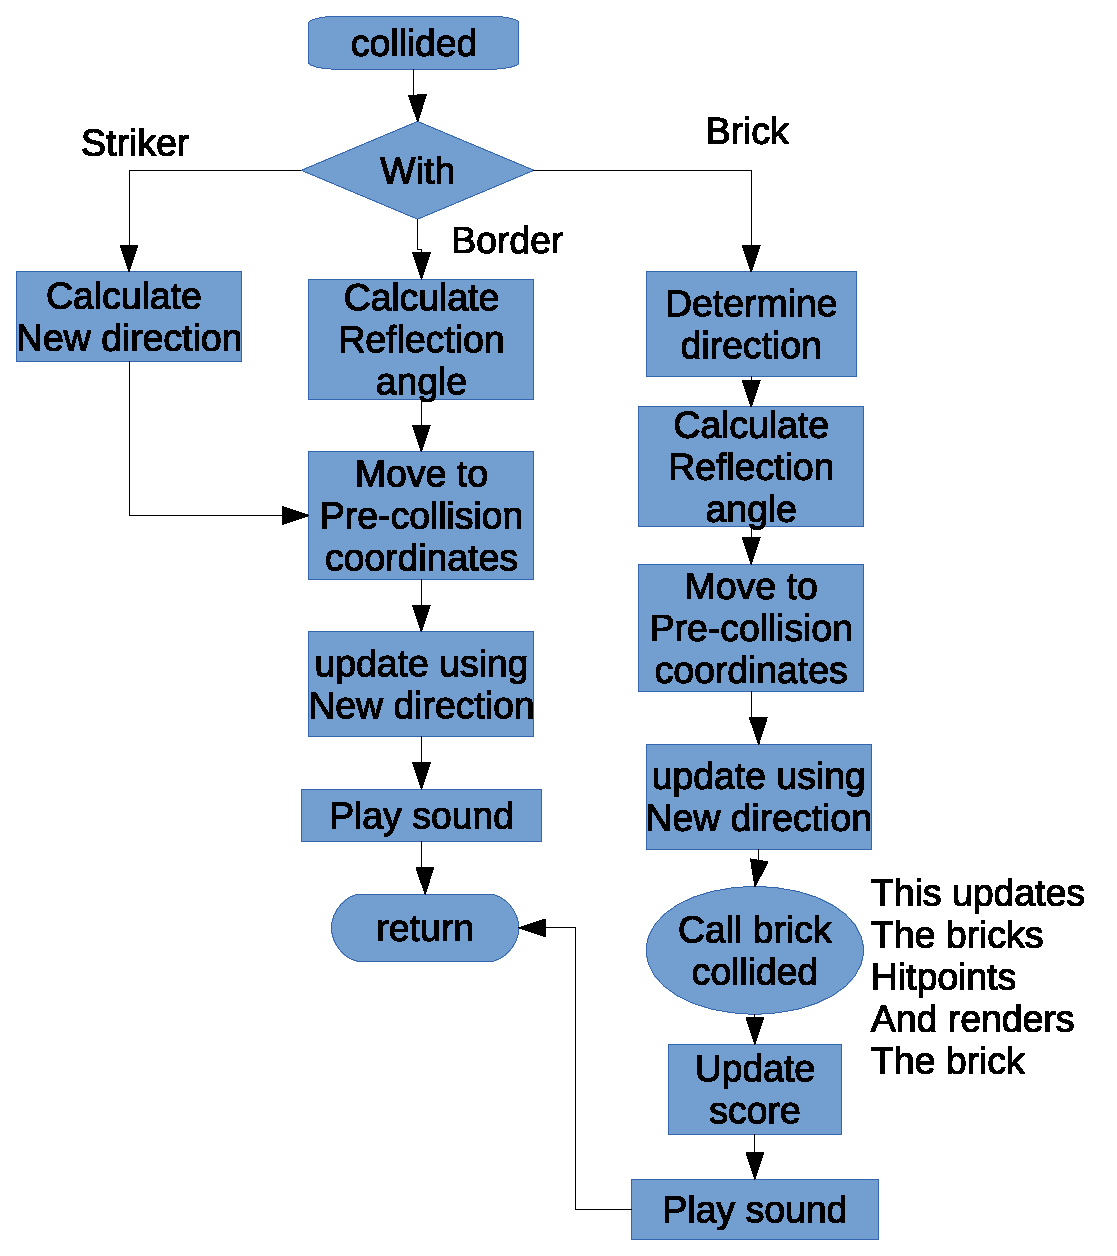
\includegraphics[scale=0.5]{pictures/ball_flow.eps}
	\caption{Program flow upon a ball collision, the redundancy in calculating the reflected
	direction when colliding with a brick is due to it being different depending on the direction
	from which the ball approached the brick.}
	\label{ball_flow}
\end{figure}

\paragraph{Striker Entity}
The striker entity polls the keystate/joystick value when updating its position. It then 
calculates a new position depending on the striker speed. When rendering, only the needed
characters are drawn instead of erasing the striker before drawing it, to maximize drawing
performance.

\paragraph{Brick Entity}
The brick entity is only updated upon a collision since it cannot move, 
